\documentclass{article} 
\usepackage[a4paper,left=20mm,right=20mm,bottom=15mm,top=15mm]{geometry}
\usepackage{amsmath} % 
\usepackage{graphicx} % Required to insert images

\title{Zama design challenge} 
\author{Purush} 
\date{\today}

\begin{document} % All begin commands must be paired with an end command somewhere
    \maketitle 
    
    \section{ Chronology of understanding} % creates a section

    To begin, I'll outline my approach to understanding the problem and devising a solution. Recognizing the importance of comprehending homomorphic encryption and its underlying mathematics, I delved into these concepts to gain a deeper appreciation of the complexity involved. This exploration also provided insights into the current and potential future benchmarks regarding latency, throughput, and implementation costs.

    With these objectives in mind, the initial three days were dedicated to studying a relevant blog post and academic paper. Although I initially started reading the paper, it quickly became apparent that I lacked the necessary mathematical foundation to grasp its contents. Consequently, I shifted focus to the blog post, using it as a starting point to familiarize myself with the essential mathematical principles. This involved consulting various papers and watching instructional videos on platforms like YouTube. However, I encountered discrepancies in the terminology and concepts presented, which led to more confusion.
    
    The root of this confusion lies in the disparity between the notions discussed. While the theory of polynomial fields resonated with me due to prior experience with Galois fields in Reed-Solomon encoding, considerable effort and time were devoted to understanding the distinctions between them. In essence, the crux of the matter can be summarized as follows:

    \begin{itemize}
      \item A polynomial has two characteristics: its length 'n' and its coefficient modulo 'q', represented as $R_q$. 
            The length 'n' is fixed, and a sample from the polynomial can be expressed as an array of 'n' numbers, each element ranging from [0, $q-1$]. 
            Therefore, the array can be represented with unsigned numbers of bit width $\lceil \log_2(q) \rceil$. 
            Although not necessary, choosing 'N' and 'Q' as powers of 2 can lead to more efficient hardware implementations.
      \item From a usage perspective, there are two fundamental operations: ADD and MULT. Additionally, 
            there is a need for a 'reduction' operation, which in this context is a power of 2 modulus.
  \end{itemize}

   \subsection{Python code}

   The code doesn't always function correctly. This could be due to an issue with the algorithm or parameter settings, or possibly due to overflow/underflow errors in the Python code (Figure \ref{fig:errored_dec1}, \ref{fig:errored_dec2} ). Interestingly, the values are generally close and approximately correct, which suggests that the problem may be related to numerical precision errors.

      \begin{figure}[hbtp] 
            \centering
            \includegraphics[width=0.8\textwidth]{errored_decryption.png} 
            \caption{Decryption error: example1} 
            \label{fig:errored_dec1}
      \end{figure}

      \begin{figure}[htpb] 
            \centering
            \includegraphics[width=0.8\textwidth]{errored_decryption2.png}
            \caption{Decryption error: example2}
            \label{fig:errored_dec2} 
      \end{figure}

      After some investigation, the rounding errors might come from the fact that \textit{rlwe\_he\_scheme\_updated.polymul()} implementation calculates the final value of multiplication thorough a final modulus and \textit{np.int64()} function. The model also encounters issues when used with parameter set C, due to the fact that the ciphertext modulo \(Q = 64\) exceeds the capacity of the signed implementation of \textit{np.int64()} in the Python model. Similar issues may arise when running the decryption algorithm with \textit{relinearization\_ver2} for Parameter set A. However, \textit{relinearization version1} operates without any issues for the same parameter set. Finally, running parameter set B in python is out of question, as (q=$2^{512}$).


    \section{Design challenge: Part 1}

    \subsection{Encryption}
    This part is to focus on encryption algorithm and propose an architecture for it. The encryption equation is given as for every message(m) one has to calculate: 
    $$
    c_t = \left( \left[ (pk0 \cdot u + e_1 + \Delta \cdot m) \right]_{R_q} ,
                 \left[ (pk1 \cdot u + e_2) \right]_{R_q} \right)  \in {R_q}\times {R_q}
    $$
    
    \begin{figure}[htp] 
      \centering
      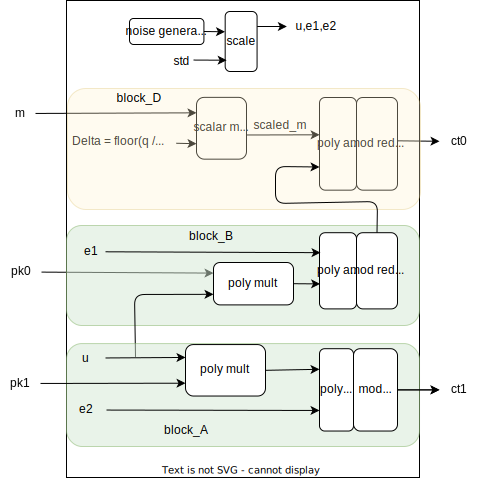
\includegraphics[width=0.6\textwidth]{FV12_encryption.png}
      \caption{System Architecture}
      \label{fig:sysarch} 
    \end{figure}

    \subsection{Analysis}
    From the given use case, we know public key tuple [pk1, pk0] is pre-computed at the host once at the beginning and is used all encryptions.

    for every $m$,
    \begin{itemize}
      \item sample: r1,r2: normal distribution in R
            \subitem u : binary, uniform distribution sample from R
      \item $block\_A$  and $block\_B$ operation is independent of $Block\_D$, provided $u$ is saved for use in $block\_B$
      \item Since q and t are constant $\Delta=\lfloor q/t \rfloor$ is also constant and can be expressed as a power of 2. 
            Hence, scaling is just a left-shift operation on the individual fields of incoming message vector m.
    \end{itemize}

In our particular case, i.e., for parameter sets A and B, (m) is left-shifted by 24 and 448, respectively. It is worth noting that even after scaling, the field elements of ($scaled\_m$) are never greater than \(q\). Therefore, no overflows occur after scaling of field values, and they can still be represented in ($\log_2(q)$) bits. In summary, reducing the latency of encryption is constrained to calculation of one $poly\_add$ function.

\subsection{Thought process}

Consider parameter set A. First we calculate, $C_1 = pk0 \cdot u + e_1$  mod q and $C_0$ = $pk1 \cdot u + e_2$ mod q. 
 $ pk0 \cdot u$ is a 128 coeffcient, polynomial multiplication. Since, it is relatively a
small number we can do it serially as done in part 2 of the challenge. 
     
Next let's calculate $C'_1 + \Delta.m$. Since, lower 24 bits of $\Delta.m$ is zero. $(e_1 + \Delta.m)$ mod q, can be done in one 8-bit adder.    
    Hence the design would be: with two serial multipliers, followed by a 32 bit adder, one of which
    is further follwed by a 8 bit adder.

    Cost of 1 polynomial serial multiplier= Polymult = 2*[(2579 LUTs + 2172 FFs)] 

    Hence the total hardware cost: 2*[2*Polymult + 32 bit adder]

    and the latency is : ~128 clock cycles.

    The serial architecture is as shown in figure \ref{fig:param_enc}. But this solution, is naive and baised towards using 
the serial multiplier in part 2 of the challenge. So note this is NOT the final solution, but might pass as A solution. 

    \begin{figure}[htp] 
      \centering
      \includegraphics[width=0.6\textwidth]{enc_param_a.png}
      \caption{System Architecture: Naive Encryption parameter set A}
      \label{fig:param_enc} 
    \end{figure}

Let's consider design for parameter set B. The polynomial size is : 16384. One obvious elimination is the above serial multiplication. In this case, we can approach the problem using number theoritic transform, which is number theory version of FFT. We know that the number of multiplications reduces from $O(N^2)$ to O(Nlog2(N)) 'scalar' multiplications and accomplishes it in log2(N) = 14 stages.

    The algorithm for polynomial multiplication would be in this case be: 

    \begin{align} 
      C'_1 &= INTT(\ NTT(Pk0)\ o\ NTT(u) ), \label{eq:2}
    \end{align}

    Where $o$ represents the is an element-wise vector multiplication in $R$ in section \ref{sec:NCC}. From equation \ref{eq:2}, we can notice that $Pk0$, is pre known and constant, hence it can be pre-calculated. So the actual hardware implementation cost is calculating INTT() and NTT(u). 

With no full understanding of NTT in number theory,  (other than  the reading reference (1) ), I guess NTT(u) is binary and still behaves as  uniform random sample ?. If that's the case, we can skip calculating NTT(u) and directly multiply u with NTT(Pk0).  

\section{Solution}
But, the final solution may look like the architecture in figure \ref{fig:param_enc_AB} (A) for parameter set A.  For parameter set B,  use 128 instances of this to realise architecture figure \ref{fig:param_enc_AB} B. I am skipping the details, for a reason that I cannot make sound reasoning without full understanding of NTT. But, the intuitively, the solution lies in dividing the 16384 long pk0 NTT transform into 128 chunks each of size 128 multiply 128 bits of the 'u'.

    \begin{figure}[htp] 
      \centering
      \includegraphics[width=0.6\textwidth]{enc_param_ab.png}
      \caption{System Architecture: Propose Encryption parameter set A}
      \label{fig:param_enc_AB} 
    \end{figure}


    \section{Design challenge: Part 2}
    This part zooms into implementation of $z = pk0 \cdot u$ part of the encrption algorithm. It gives us some idea of the complexity of polynomial
    multiplication even though one of the parameters \textit{u} is just one-bit wide.

    So the hardware needs to do polynomial multiplication of $u \in R_2$ with  $p \in R_q$ to produce a result  $z \in R_q$.
    The fields in/out through an AXI stream interface. 

    \subsection{Algorithm: Negative wrapped convolution}\label{sec:NCC} 
    (NOTE: I wrote this before getting actual name for the method, in reference (1). I choose to let it stay to for the sake of completeness.)
    Polynomial multiplication can be seen as circular convolution coeffcients of the two polynomials. 
    Say N=4, two polynomials  A(x) and B(x) are to be multiplied, the final result $C(x)$ is given as below.

    \begin{align}
      f(x) \ast g(x) &= \sum_{k=0}^{N-1} f(k) \cdot g((n-k) \mod N) \\
      A(x) &= a_0 + a_1x + a_2x^2 + a_3x^3 \\
      B(x) &= b_0 + b_1x + b_2x^2 + b_3x^3 \\
      C(x) = P(x) \times Q(x) &= c_0 + c_1x + c_2x^2 + c_3x^3 + c_4x^4 + c_5x^5 + c_6x^6 \\
      C(x) &= c_0 + c_1x + c_2x^2 + c_3x^3 - c_4 - c_5x - c_6x^2\ \ \   subsituting\ \ \ X^4 = -1 
    \end{align}

    Where,
    \begin{align}
      c_0 &= a_0 \cdot b_0 \\
      c_1 &= a_0 \cdot b_1 + a_1 \cdot b_0 \\
      c_2 &= a_0 \cdot b_2 + a_1 \cdot b_1 + a_2 \cdot b_0 \\
      c_3 &= a_0 \cdot b_3 + a_1 \cdot b_2 + a_2 \cdot b_1 + a_3 \cdot b_0 \\
      c_4 &= a_1 \cdot b_3 + a_2 \cdot b_2 + a_3 \cdot b_1 \\
      c_5 &= a_2 \cdot b_3 + a_3 \cdot b_2 \\
      c_6 &= a_3 \cdot b_3 \\
    \end{align} 
    
    \begin{align}
      C(x) &= (c_0-c_4) + (c_1- c_5)x + (c_2- c_6)x^2 + c_3x^3  \\
      C(x) &= s_0 + s_1x + s_2x^2 + s_3x^3  \\
      s_0 &= (a_0 \cdot b_0 - a_1 \cdot b_3 - a_2 \cdot b_2 - a_3 \cdot b_1 )\ mod Q\\
      s_1 &= (a_0 \cdot b_1 + a_1 \cdot b_0 - a_2 \cdot b_3 - a_3 \cdot b_2 )\ mod Q\\
      s_2 &= (a_0 \cdot b_2 + a_1 \cdot b_1 + a_2 \cdot b_0 - a_3 \cdot b_3 )\ mod Q\\
      s_3 &= (a_0 \cdot b_3 + a_1 \cdot b_2 + a_2 \cdot b_1 + a_3 \cdot b_0 )\ mod Q\\
    \end{align} 
    
    To realise the implementation in hardware, we set N partial product calulators (pprod). Each pprod, starts one clock cycle
    after the previous one and continues to calculate partial product for N clock cycles. Pictorially, it can be shown as in figure \ref{fig:multiplier}. 
    
    pProd0 is active from clk0 to clk3, pProd1 is active from clk1 to clk4, and so on. 
    The final results which are C(0),C(1),C(2),C(3), are read out start clk4,clk5, clk6 and clk7 respectively.

    \begin{figure}[htp] 
      \centering
      \includegraphics[width=0.6\textwidth]{multiplier_func.png}
      \caption{Multiplier dataflow}
      \label{fig:multiplier} 
    \end{figure}

    Figure \ref{fig:multiplier}.c show calculate C(x) through matrix multiplication. The structure of the matrix is similar to circular 
    convolution matrix except for the sign changes that occurs due to polynomial division.

    In summary, it can be seen serial polynomial multiplication happens in N clock cycles. In order to achieve non-stop streaming operation, two such
    multipliers are instantiated as shown in \ref{ref:multiplier_top} each operating on alternate packets.

    \begin{figure}[htp] 
      \centering
      \includegraphics[width=0.6\textwidth]{multiplier_top.png}
      \caption{Multiplier top instance}
      \label{fig:multiplier_top} 
    \end{figure}

    \subsection{Simulation}
    The simulation environment is abysmally simplistic, in order meet the task completion deadline. Ideally, cocotb would have
    been used for faster checking. But that would have meant mandatory use of cocotb for even simple code sanity check. 

    The code in \textit{tb\_multiplier.sv} instantiates \textit{multiplier\_top} by default. This instantiates two multipliers 
    and streams three packets back-to-back. To test only the single multipler one can just change the instance name to \textit{multiplier} 
    and comment extra packets being sent. 

    \subsection{Synthesis}
    To meet this goal few extra blocks were quickly added intentful code writing. 
    This includes an AXI stream lfsr generating random samples and the configurable packet size N, as source for P and U 
    ports. For Z output interface writes into a simple AXI memory. 
    But synthesising this lead to total optimization of the built logic. The synthesis tool ultimately optimises every away.
    This was a wasted use of time, writing system verilog code with interfaces passed on to tasks exposed some quirks of the tool that were previously unknown to me.  
    
    A simple synthesis instantiating the single multiplier to run at 172 MHz, with 2579 LUTS and 2172 FFs. This is the case, when meeting timing for the entire design including the pins is considered. 
  
    \begin{figure}[htp] 
      \centering
      \includegraphics[width=1\textwidth]{synthesis_results.png}
      \caption{Synthesis results}
      \label{fig:syn_result} 
    \end{figure}
       
    \section{What if...more time was given?}

    As the saying goes, with if's and buts one can build castles in the air. But being pragmatic, 
    these are the top priorities in the to do list
    \begin{itemize}
      \item Understand the use of DSP48E2 block's multiplixing modes. 
      \item Write a more complete test bench for the design and check random constrained cases and also bit width growth. Perhaps with cocotb.
      \item Spend time in reading and understanding  in detail basic algorithms, Barret's algorithm for reduction. NTT for multiplication.
      \item Revisit code for cleanness, and do some refactoring.
    \end{itemize}

\section{References}
\begin{itemize}
  \item [Number theory] https://eprint.iacr.org/2024/585.pdf
  \item [FAB](https://bu-icsg.github.io/publications/2023/fhe\_accelerator\_fpga\_hpca2023.pdf)
  \item [Post-Quantum Cryptographic Hardware Primitives](https://arxiv.org/pdf/1903.03735)
  \item [Blog post](https://bit-ml.github.io/blog/post/homomorphic-encryption-toy-implementation-in-python)
  \item [Fast Arithmetic Hardware Library For RLWE-Based Homomorphic Encryption](https://ascslab.org/papers/he-library.pdf)
  \item [RISE](https://arxiv.org/pdf/2302.07104)
  \item [MAD](https://bu-icsg.github.io/publications/2023/Agrawal\_MICRO\_2023.pdf)
\end{itemize}


\end{document} % This is the end of the document
